% !TEX root = PREN2_Dokumentation.tex
\section{System-Spezifikation}\label{SystemSpezifikation}
\subsection{Systemübersicht}
\subsubsection{Systemarchitektur}
\begin{figure}[H]
    \centering
    \includegraphics[width=1\textwidth]{images/systemoverview.png}
    \caption[Systemarchitektur]{Systemarchitektur,\\ Quelle: Autor}
    \label{img: Systemarchitektur des Projektes}
\end{figure}
\newpage
\subsubsection{Kontextdiagramm}\label{Kontextdiagram}
\begin{figure}[H]
    \centering
   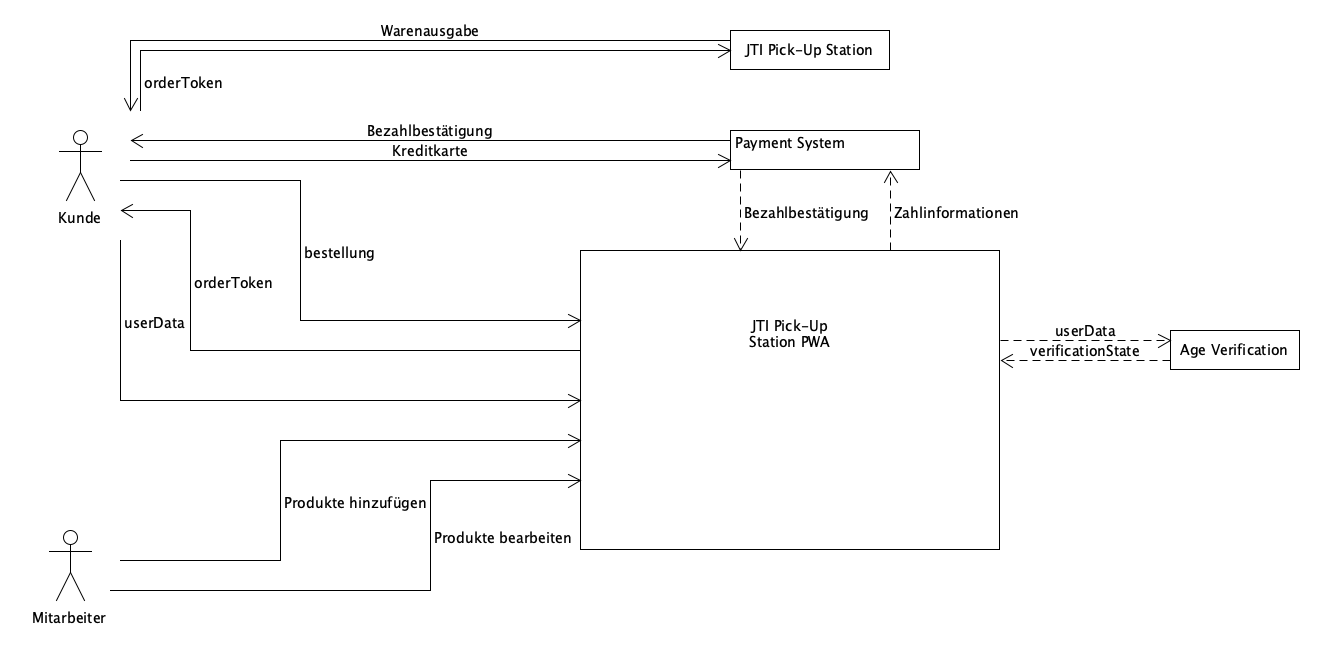
\includegraphics[width=1\textwidth]{images/kontextdiagramm.png}
    \caption[Kontextdiagramm]{Kontextdiagramm,\\ Quelle: Autor}
    \label{img: Kontextdiagramm des Projektes}
\end{figure}
\newpage
\newpage
\subsection{Architektur und Designentscheide}

\subsubsection{Modelle und Sichten}
In diesem Projekt wird zwischen zwei verschiedenen Sichten unterschieden:
\begin{itemize}
    \item \textbf{Kunde} Es handelt sich dabei um die Person, welche in der \ac{PWA} Produkte bestellt und diese abholt. 
    \item \textbf{Administrator} Dem Administrator ist es möglich, Produkt hinzuzufügen, zu verändern oder auch zu löschen. 
    \item \textbf{Programmierer: } Dieser konzipiert und realisiert die Applikation gemäss den Anforderungen des Auftraggebers.
\end{itemize}
\subsubsection{Daten (Mengengerüst und Strukturen)}
\paragraph{Datenbankschema}
Das Datenbankschema wurde von Intelij generiert. 
\begin{figure}[H]
    \centering
    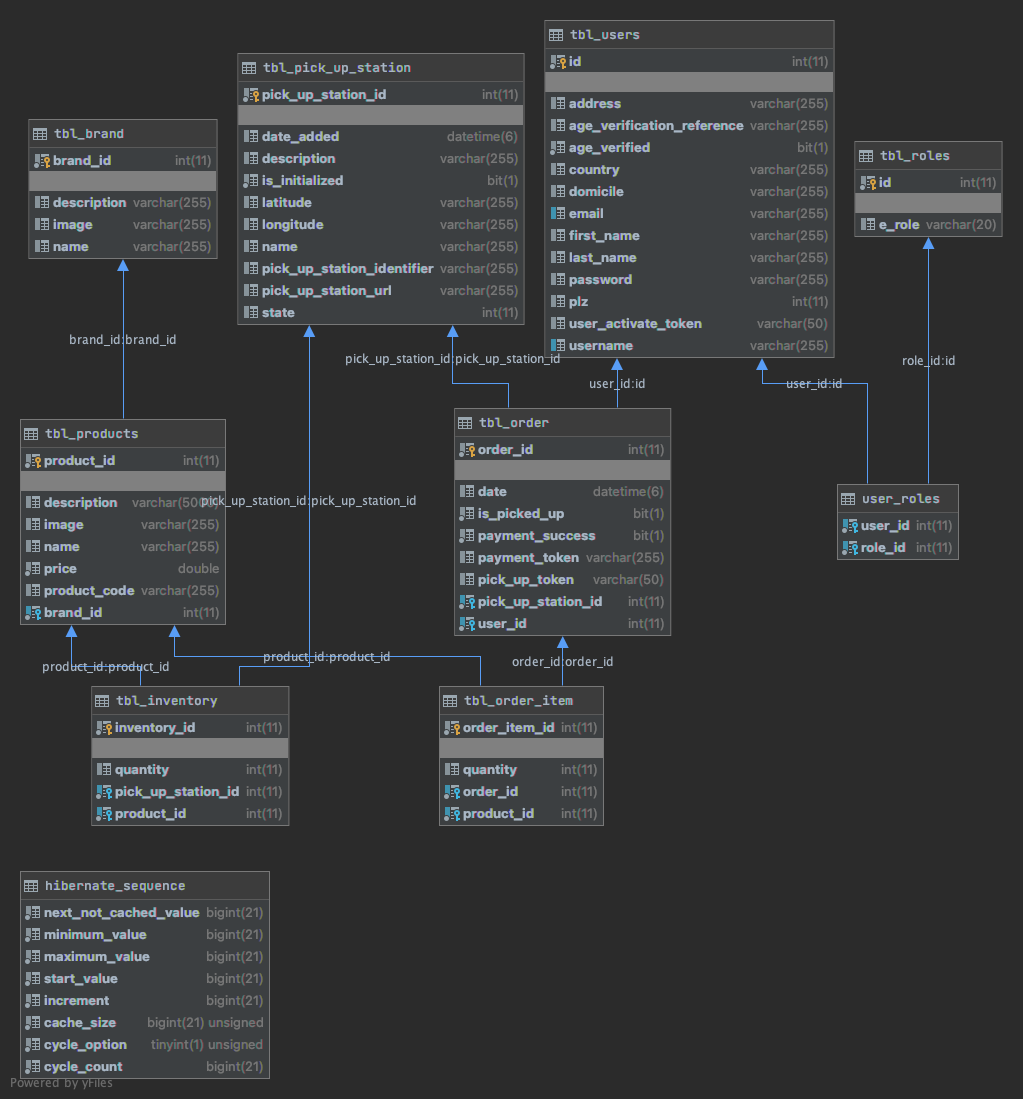
\includegraphics[width=1\textwidth]{images/databaseSchema.png}
    \caption[Datenbankschema]{Datenbankschema, Quelle: Autor}
    \label{img: datebankschema}
\end{figure}
\subsubsection{Entwurfsentscheide}
\paragraph{Frontend}
\subparagraph{Technologien}
\subparagraph{Projektstruktur}
\begin{figure}[H]
	\centering
	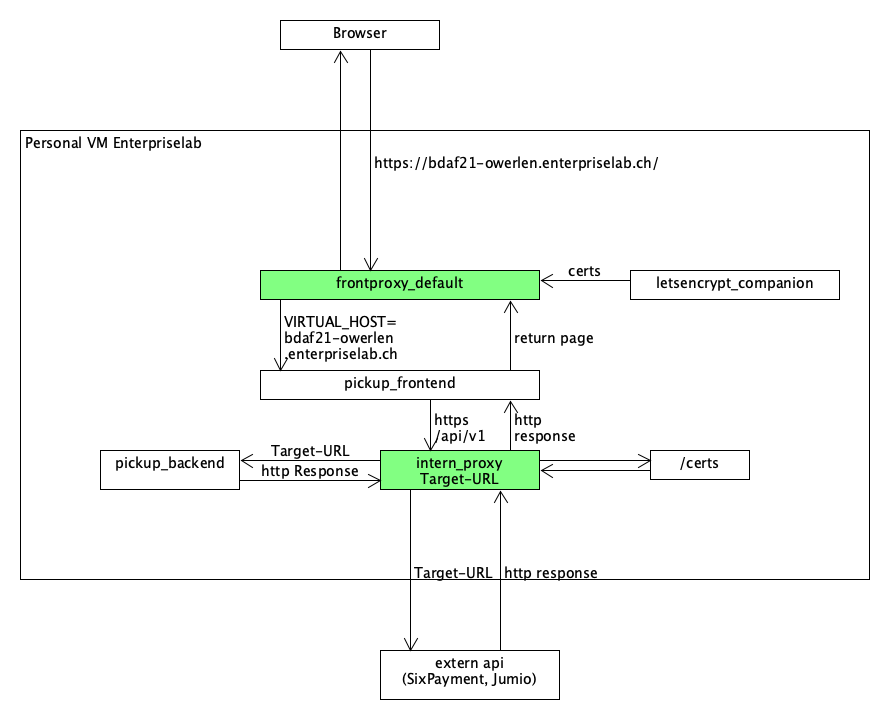
\includegraphics[width=1\textwidth]{images/requestHandling.png}
	\caption[Aufbau Produktives System]{Aufbau Produktives System, Quelle: Autor}
	\label{img: prodSystem}
\end{figure}
\paragraph{Backend}
\subparagraph{Spring Boot}
Für die Backendentwicklung wurde Spring Boot in der Version 2.3.4 genutzt.

\subparagraph{Data Transfer Object}\label{DTO}
Es handelt sich hier um ein Enterprise Application Architecture Pattern von Martin Fowler. Genauer handelt es sich um ein Distribution Pattern. \\
Durch den Einsatz dieses Patterns können mehr Daten mit einem Aufruf übertragen werden. Ein weiterer Vorteil ist die klare Trennung zwischen zu serialisierendem Objekt und dem Domain Model. In der Regel wird ein Assembler genutzt, um das DTO auf das Domain Model zu mappen. [\cite{dtoFowler}]
\begin{figure}[H]
	\centering
	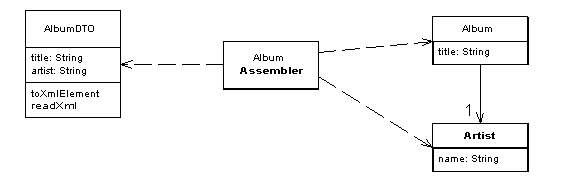
\includegraphics[width=1\textwidth]{images/dtoSketch.png}
	\caption[DTO Klassendiagramm von Martin Fowler]{DTO Klassendiagramm von Martin Fowler,\\ Quelle: \cite{dtoFowler}}
	\label{img: dtoFowler}
\end{figure}
\subparagraph{\ac{HATEOAS}}
In diesem Projekt stand der Einsatz des DTO-Pattern jedoch im Konflikt mit der REST-Abstufung von Leonard Richardson und dem von ihm entworfenen Richardson Maturity Model. Gemäss diesem sollen Daten von einem anderen Domain Model als Hyperlink zurückgegeben werden, um das höchste Level zu erreichen. Somit liefert jeder Aufruf nur das angeforderte Modell zurück. Das Data Transfer Object Pattern dient somit nur zur Abgrenzung zwischen dem zu sendenden Objekt und dem Domain Model. 

\begin{figure}[H]
	\centering
	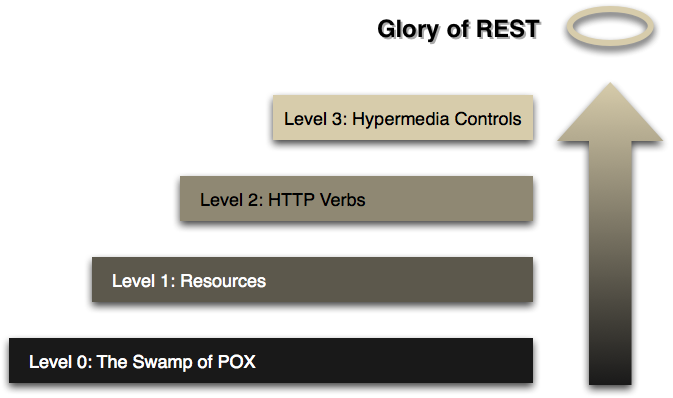
\includegraphics[scale=0.3]{images/richardsonMaturity.png}
	\caption[Richardson Maturity Model]{Richardson Maturity Model,\\ Quelle: \cite{richardsonMaturity}}
	\label{img: richardsonMaturity}
\end{figure}
Dabei wurde auf REST-Level 3 hingearbeitet und entsprechend mit HATEOAS gearbeitet. Dadurch kann das Backend weiter vom Frontend getrennt werden, da bei eine Anpassung der URL auf dem Server keinen Einfluss auf die Funktionalität des Clients hat. Zudem kann die Verständlichkeit der API verbessert und ein Erweitern vereinfacht werden. [\cite{richardsonMaturity}]
\paragraph{Datenbank}
Die Datenbank wird durch die Spring Data JPA aus den Entities in diesem Projekt erstellt. 
\paragraph{Konfigurationen}
\subparagraph{Frontend}

\newpage
\subparagraph{Backend}
\newpage
\subsection{Schnittstellen}

\subsubsection{Externe Schnittstellen}
\paragraph{REST API}
\subparagraph{API-Dokumention}
Die Spring Doc ermöglicht eine sehr einfache und schnelle Dokumentation von REST-API basierend auf der OpenAPI Spezifikation. Um die Dokumentation anzuzeigen, wird das Open Source Tool Swagger UI genutzt. Hiermit lässt sich eine dynaOnlinehe API-Dokumentation als HTML-Page erstellen. 
\begin{figure}[H]
	\centering
	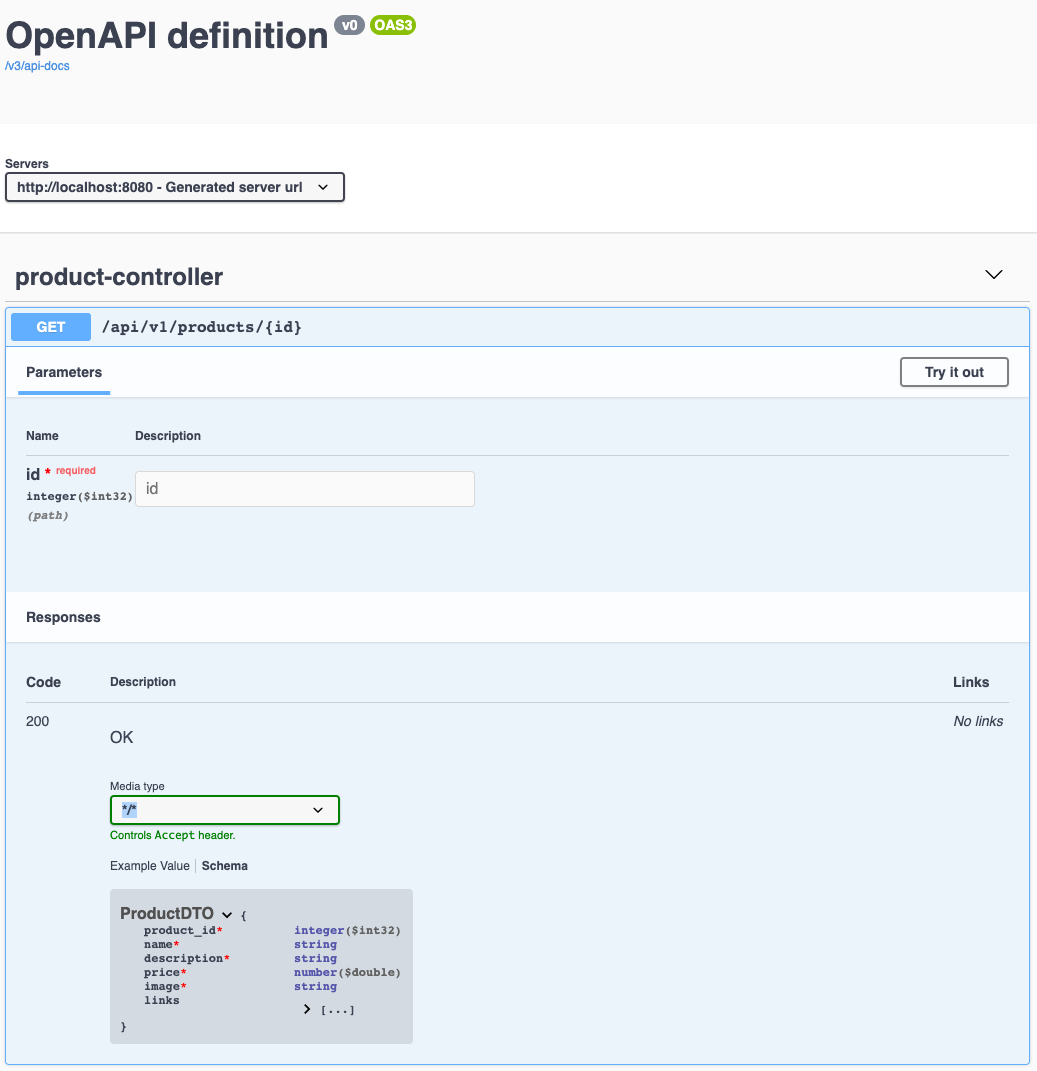
\includegraphics[scale=0.3]{images/swaggerui.png}
	\caption[Ausschnitt aus der Swagger Dokumentation]{Ausschnitt aus der Swagger Dokumentation,\\ Quelle: Autor}
	\label{img: swaggerUI}
\end{figure}
\subsubsection{Benutzerschnittstellen}
Auf ein Beschreiben der Benutzerschnittstelle wird an dieser Stelle verzichtet. 
\subsection{Environment-Anforderungen}\label{environmentanforderungen}
\subsubsection{Hardware}
Folgende Hardware wurde für diese Applikation verwendet und kann als ausreichend betrachtet werden:
\begin{itemize}
	\item CPU: Intel(R) Xeon(R) CPU E5-2630 v4 @ 2.20GHz
	\item RAM: 4GB
\end{itemize}
\subsubsection{Software}
Die ganze Applikation läuft auf virtuellen Maschine, auf der folgendes Betriebssystem installiert ist:
\begin{itemize}
	\item Ubuntu v. 20.04.01
	\item Docker v. 19.03.8
\end{itemize}
\subsubsection{Software}
\paragraph{Browser}
Die Software wurde auf den folgenden Browsern getestet. 
\begin{itemize}
	\item Safari 12
	\item Chrome 90
\end{itemize}
\newpage